


\subsection{Ordenamiento de arreglos}
Al ordenar los arreglos unidimensionales, con los algoritmos Quick sort, Merge sort y la función de sort propia de C++, se obtuvieron los siguientes resultados en la muestra de 1000 elementos:
\begin{figure}[H]
    \centering
    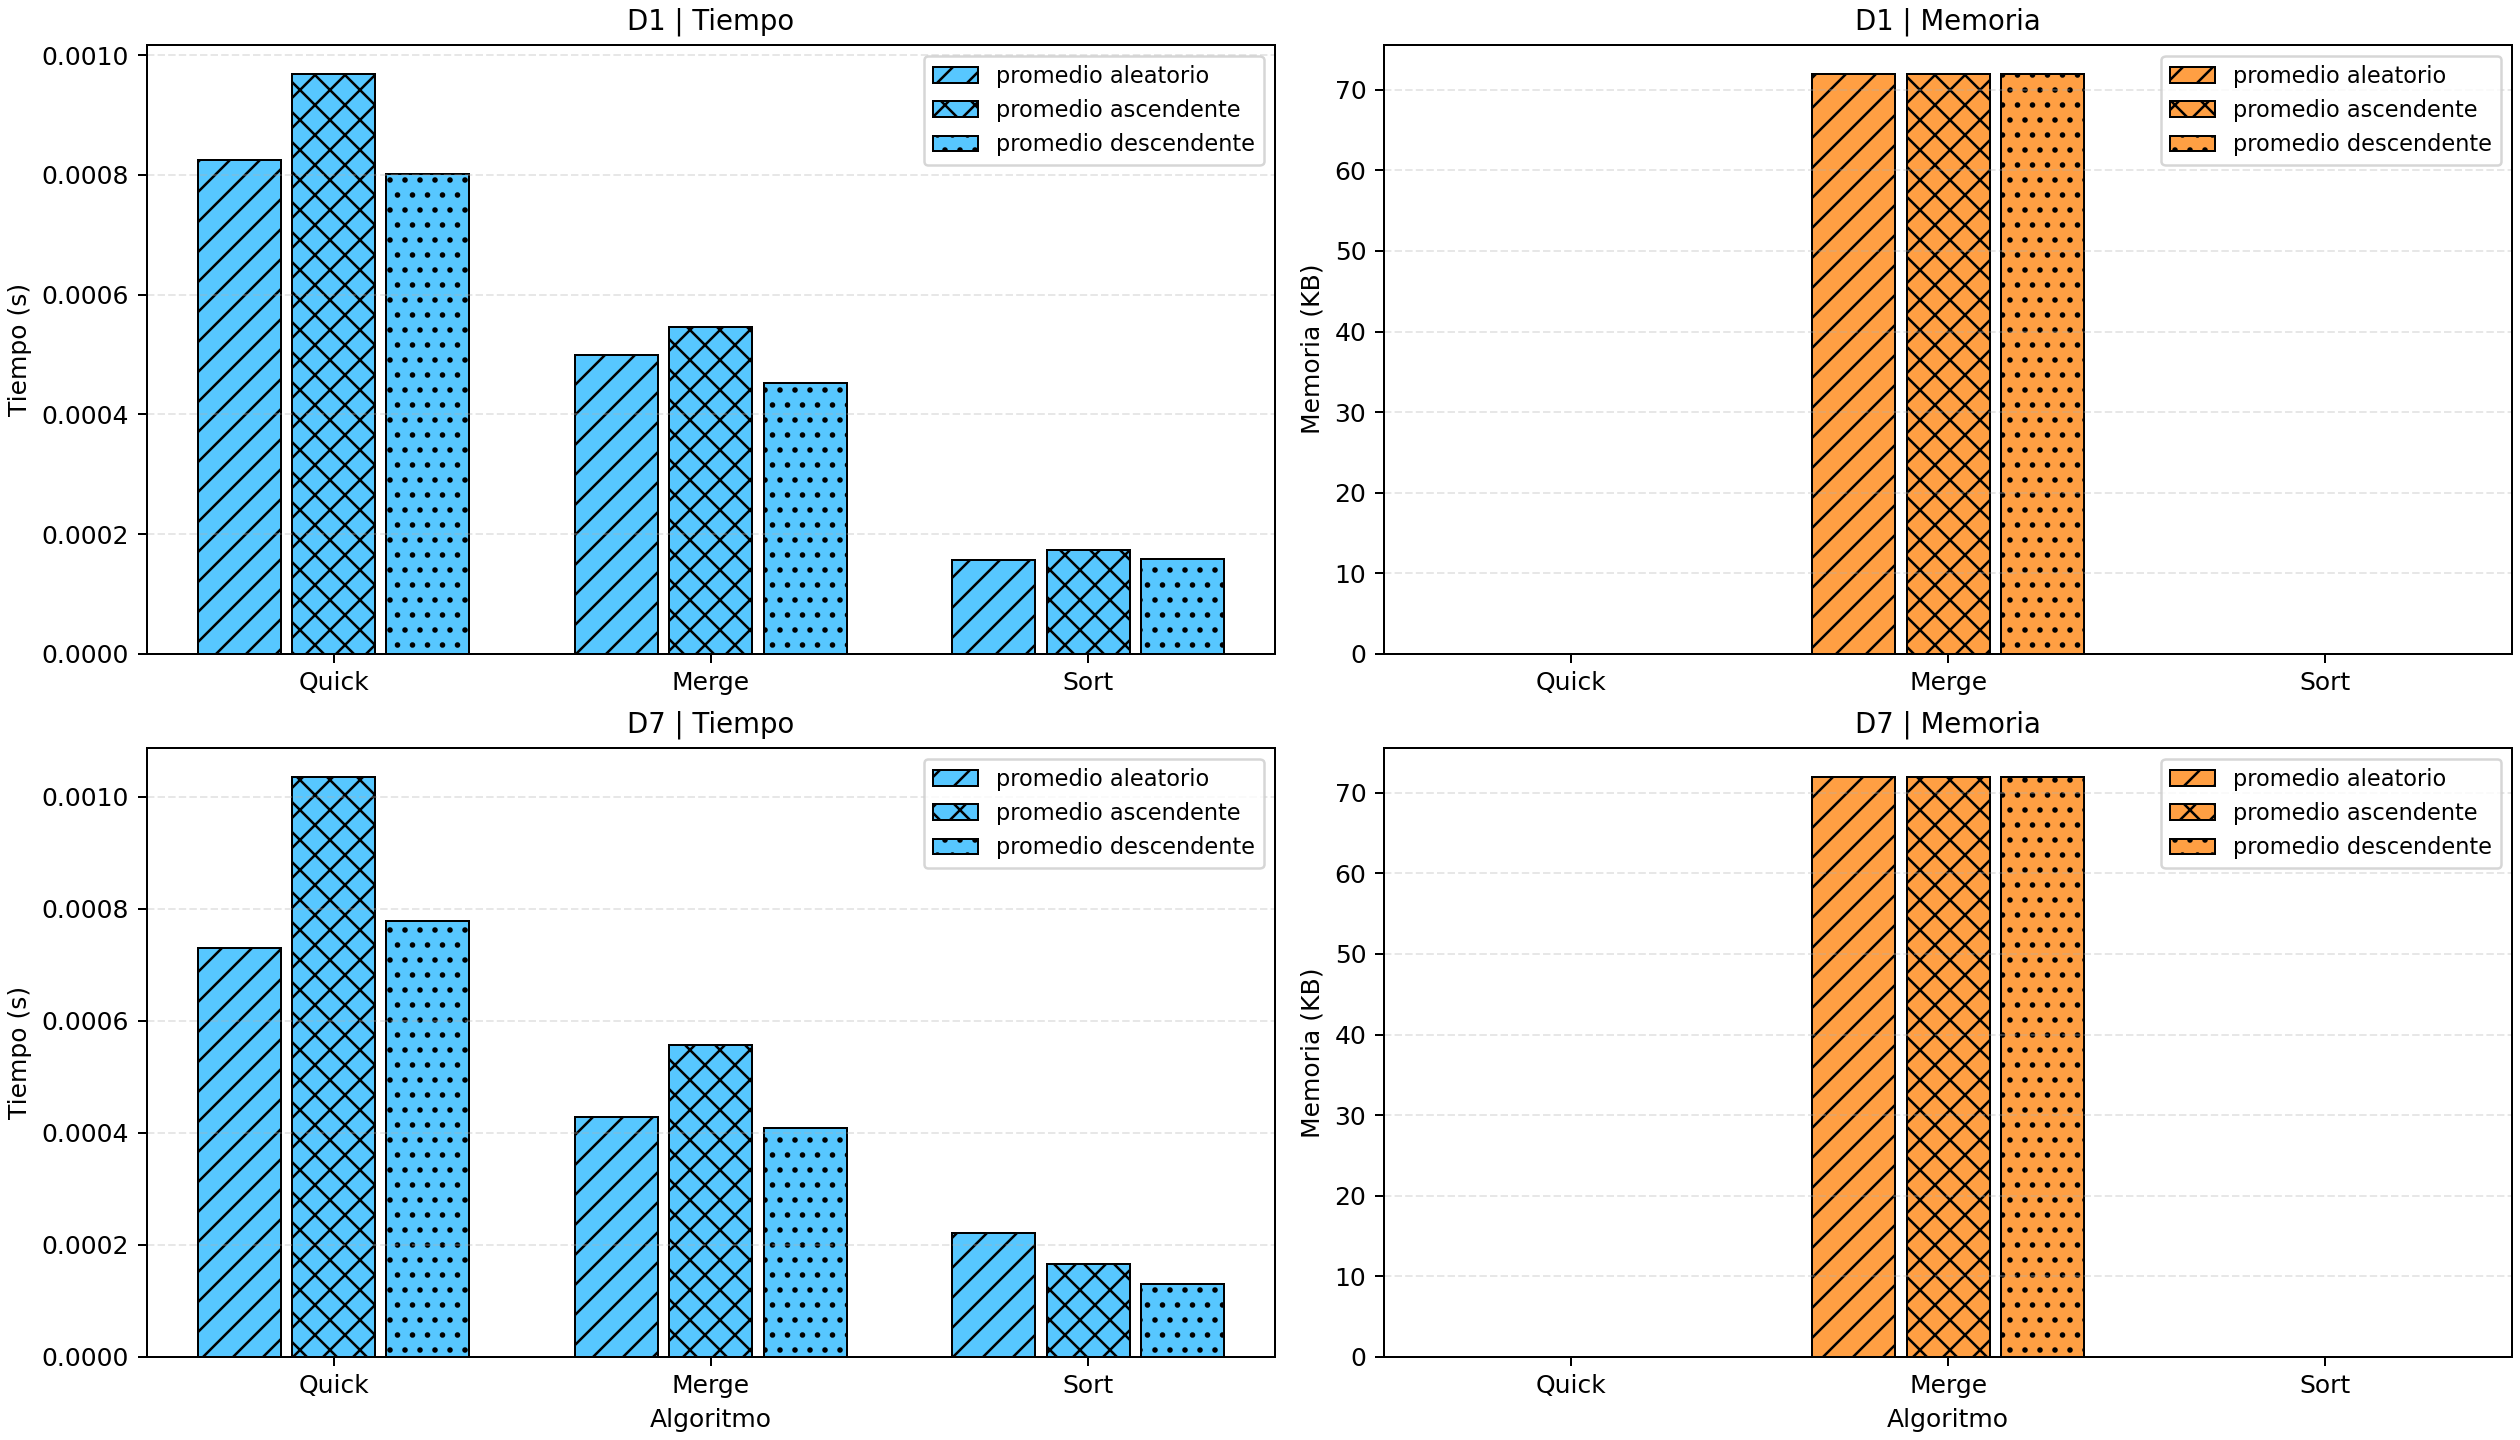
\includegraphics[width=0.9\textwidth]{../../code/sorting/data/plots/sorting_plots_size_1000_by_algorithm_type_avg_cases.png}
    \caption{Algoritmos de ordenamiento lineal (promedio de los 3 casos) para tamaño n =1000}
\end{figure}

Cómo se puede ver, para un tamaño de muestra de 1000 elementos, el tiempo de resolución de los elementos es parecido para los casos ascendentes, aleatorios y descendentes, mientras que Quick se demoró considerablemente más que Merge y Sort. En cambio, el uso de memoria de Quick y Sort fueron prácticamente nulos, mientras que Merge usó en todo caso alredero de 70Kb de memoria.

Esto es acorde al tiempo y espacio aproximados de cada algoritmo, ya que los 3 algoritmos tienen un tiempo promedio $O(n logn)$, pero el cambio radica en el peor tiempo de ejecución, ya que Quick es $O(n²)$, mientras que Merge y std::Sort son $O(n log n)$

Para el tamaño, ya que std::Sort y Quick son algoritmos prácticamente in-place, se ve que la memoria usada es casi nula, mientras que Merge usa un espacio de $O(n)$

Debido a que para mayor cantidad de elementos, este comportamiento se mantiene, se omitirá habla de mayores tamaños.


\begin{figure}[H]
    \centering
    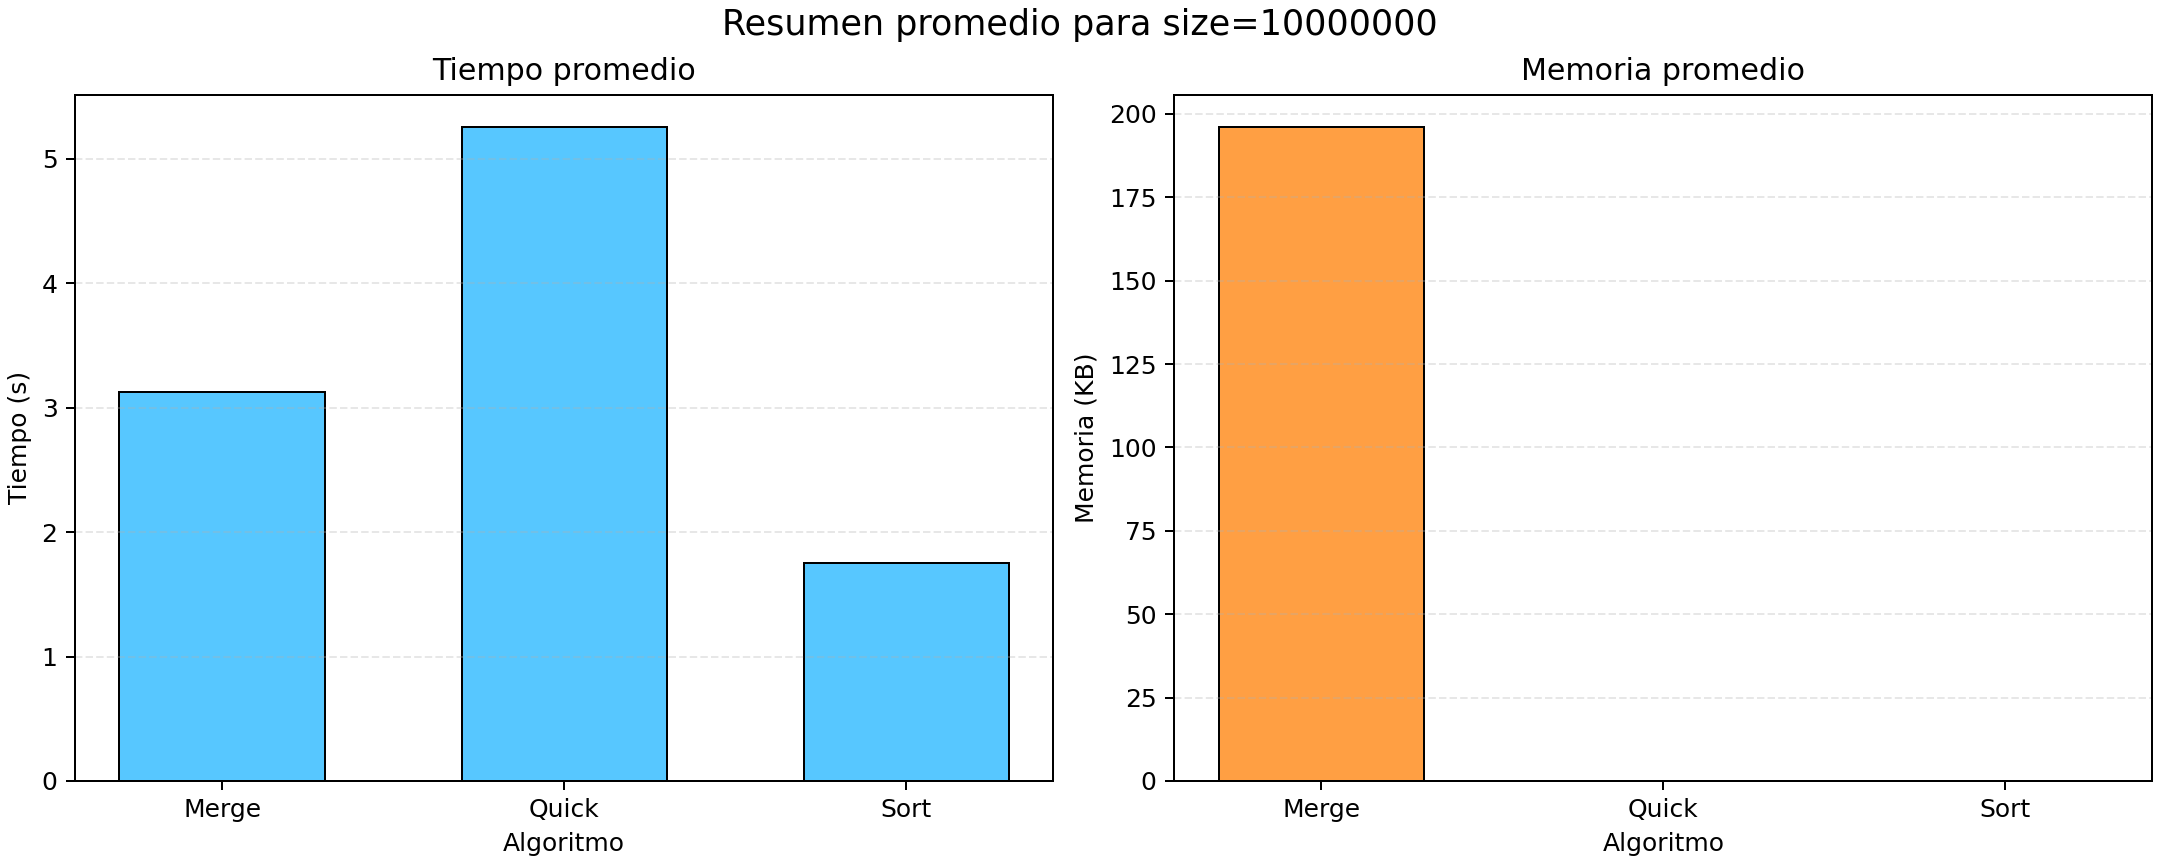
\includegraphics[width=0.9\textwidth]{../../code/sorting/data/plots/sorting_summary_size_10000000.png}
    \caption{Algoritmos de ordenamiento lineal (promedio de los casos) para tamaño n =10000000}
\end{figure}

Para una muestra de 10000000 de elementos, se observa que el orden en tiempos de ejecución se sigue manteniendo, mientras que la memoria usada por Merge subió a los 250KB, en std::Sort aumentó de forma leve y que Quick sigue siendo in-place.

Esta es una fiel representación de la descripción de cada algoritmo, ya que Quick Sort demora más pero casi no usa memoria, Merge demora menos que Quick, a cambio de usar una memoria igual a la cantidad de elementos, y std::Sort está constantemente buscando cuál es el mejor subalgoritmo para seguir, por lo que siempre tendrá mejores resultados que los otros dos.


\newpage
\subsection{Multiplicación de matrices}

Al multiplicar las matrices con los algoritmos Naive y Strassen, se obtuvieron los siguientes resultados para n = 256, osea, 2 matrices de 256 elementos cada una:

\begin{figure}[H]
    \centering
    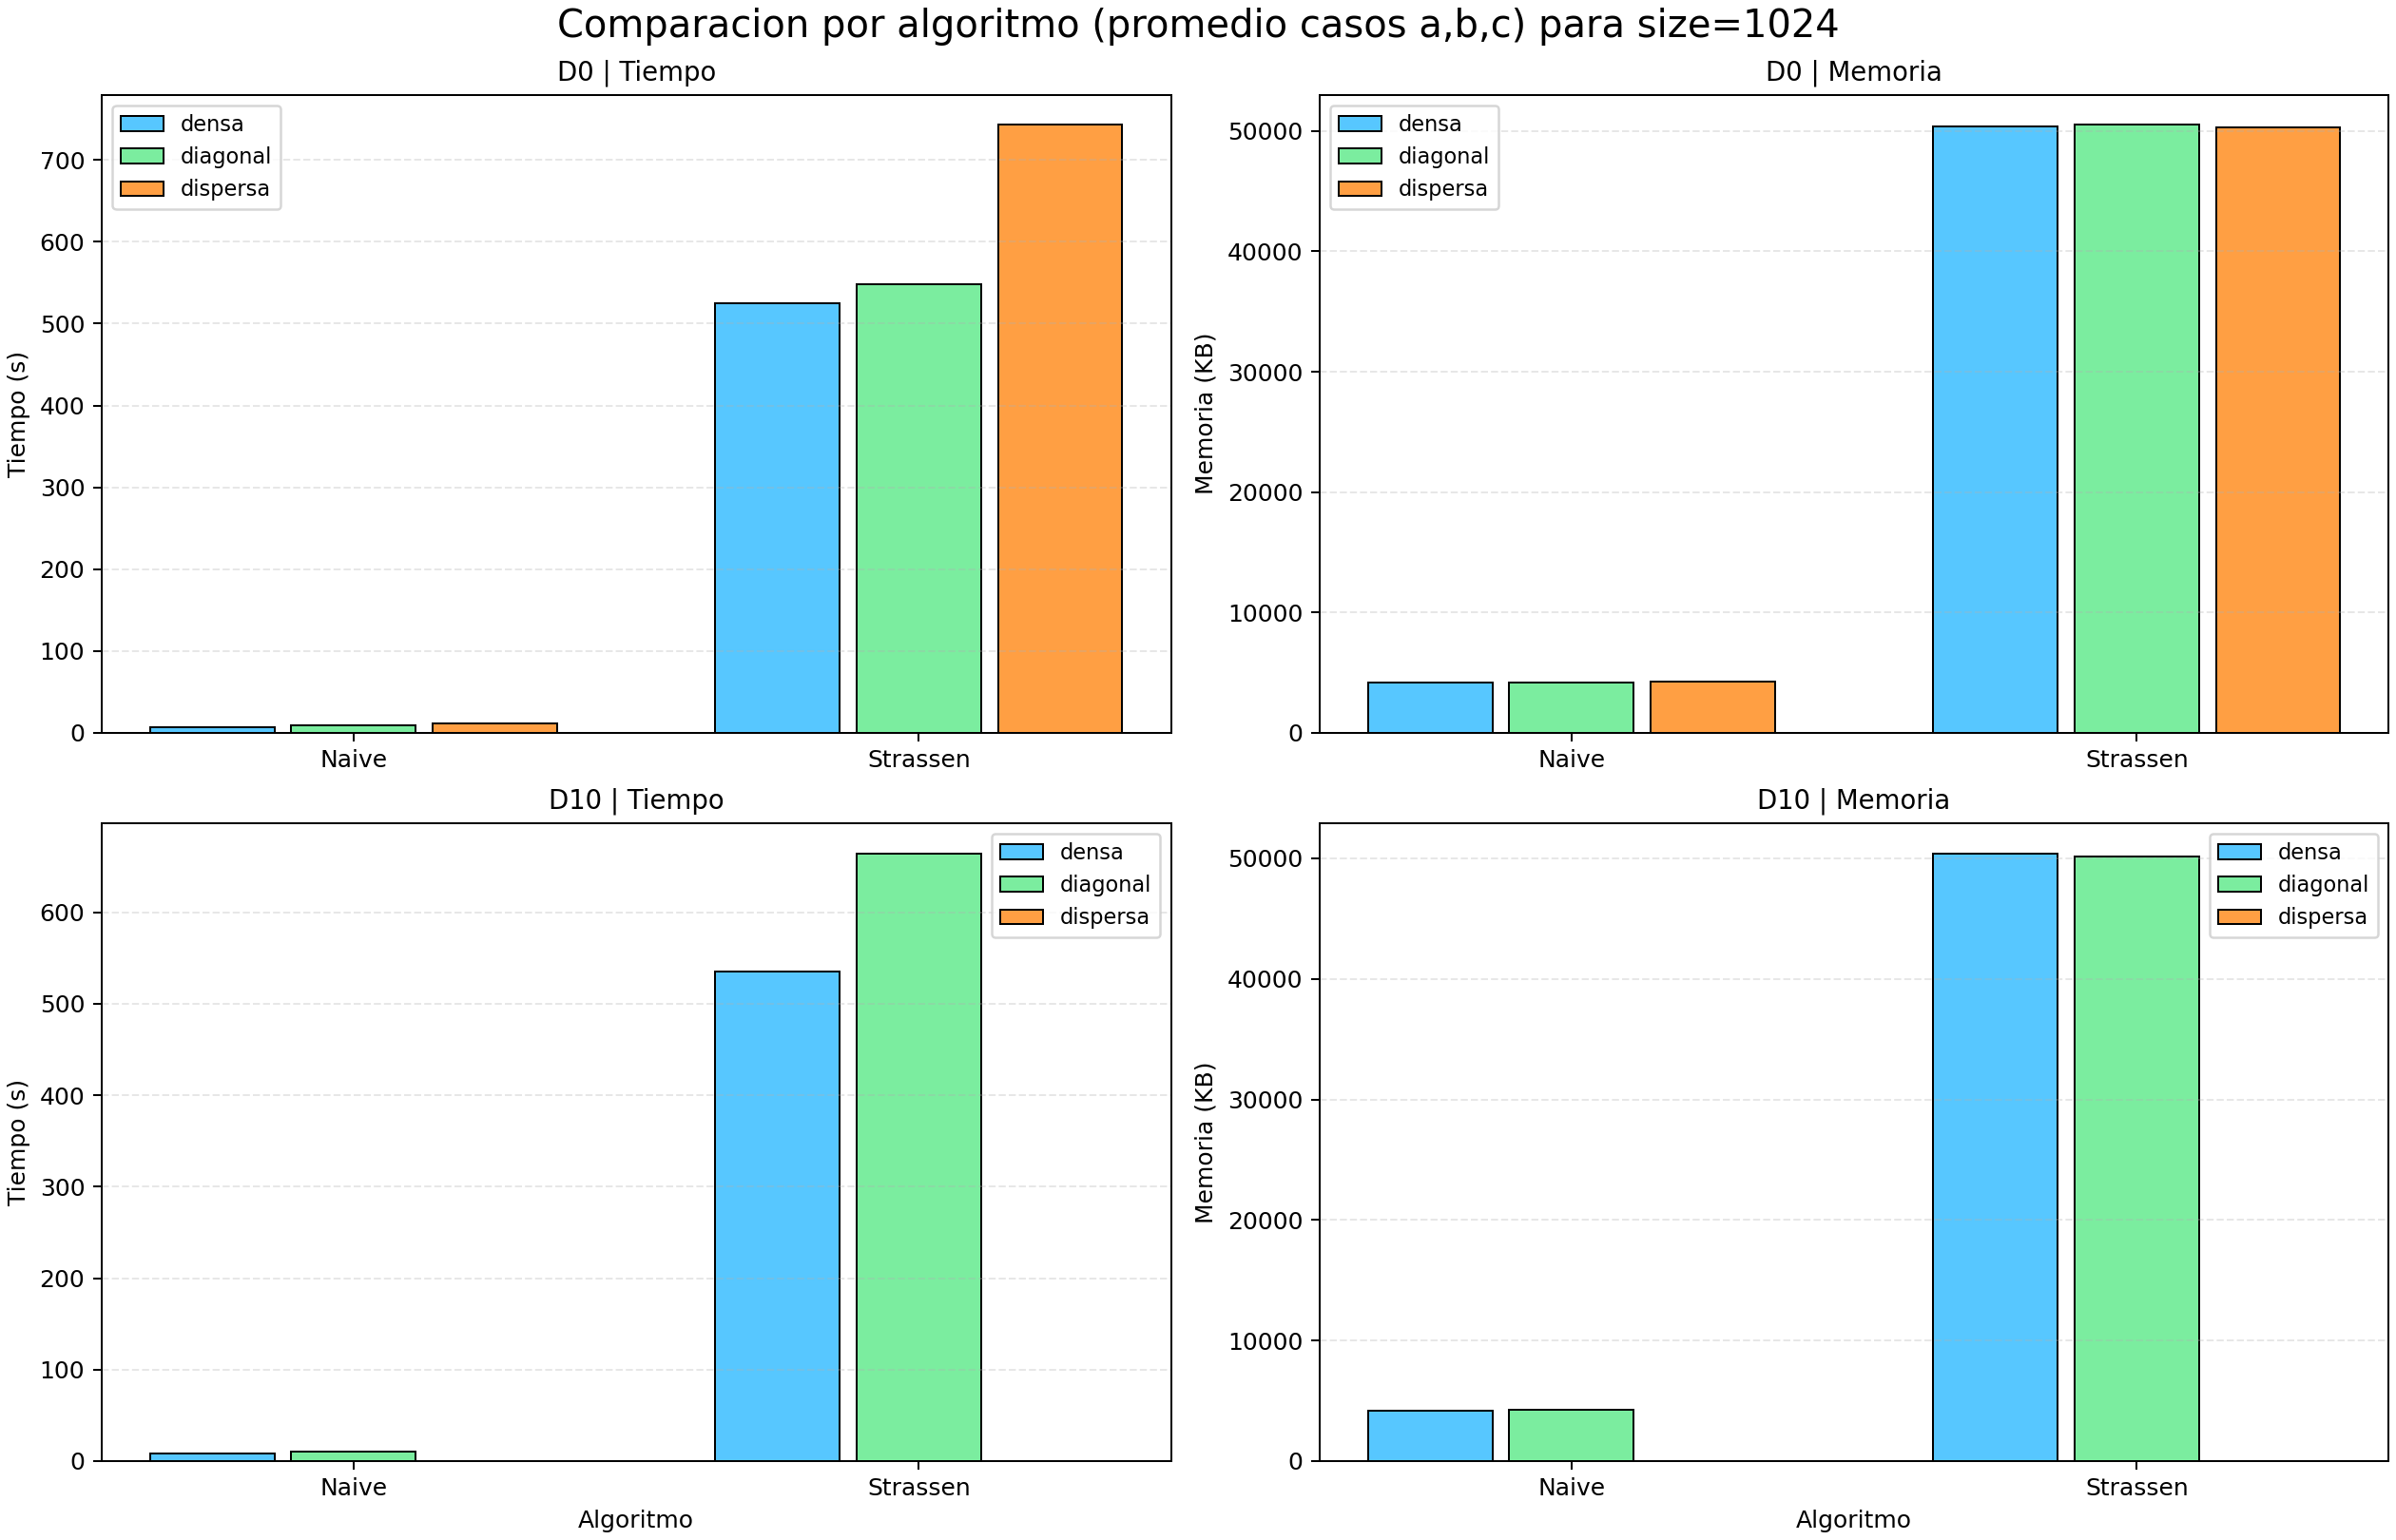
\includegraphics[width=0.9\textwidth]{../../code/matrix_multiplication/data/plots/matrix_plots_size_1024_by_algorithm_kind_avg_cases.png}
    \caption{Algoritmos de multiplicación de matrices (promedio de los casos) para tamaño n =1024}
\end{figure}

En la tabla, se puede observar que Naive usa mucho menos tiempo y espacio que Strassen, aunque el primero sea $O(n³)$ y el segundo sea $O(n^{2.87})$, lo que se contradice.

Los tiempos en Naive van en aumento lineal entre densa, diagonal y dispersa, lo que hace sentido debido a que cada vez sube más la cantidad de elementos a procesar, mientras que en Strassen hay un salto significativo en la diagonal y la dispersa, ya que aquí, la diferencia de elementos no nulos con Strassen hace que se realice mucho más esfuerzo.

En cuanto a espacio, se puede ver que tanto para D0 como D10, se obtiene un uso similar entre casos, ya que el algoritmo de Strassen realiza múltiples copias de las submatrices durante la recursión, lo que resulta en un consumo de memoria de $O(n²)$ independientemente de la densidad de la matriz. Por el contrario, Naive mantiene un uso de memoria prácticamente constante, ya que solo almacena la matriz resultado sin crear estructuras intermedias adicionales.

El mismo comportamiento se ve para matrices más pequeñas, por lo que se ignorarán. Además, debido al tiempo de ejecución, no se realizó el caso de prueba dispersa para D10, pero se asume que tendŕa un comportamiento parecido al de D0.

La contradicción de tiempo sólo se puede justificar con una mala implementación del algoritmo de Strassen, ya que por ejemplo, no recibe la matriz cómo referencia, si no que la recibe cómo parámetro, incrementando de forma exponencial el tiempo y la memoria utilizados.